\documentclass[crop=false]{standalone}
% --- ПРЕАМБУЛА ДЛЯ ПОДДЕРЖКИ РУССКОГО ЯЗЫКА И МАТЕМАТИКИ ---
\usepackage[T2A]{fontenc}
\usepackage[utf8]{inputenc}
\usepackage[russian]{babel}
\usepackage{amsmath}
\usepackage{geometry}
\usepackage{amssymb}
\usepackage{graphicx}
\usepackage{float}
\usepackage{import}
\geometry{a4paper, top=2cm, bottom=2cm, left=2cm, right=2cm}
\newcommand{\sidecomment}[1]{\marginpar{\raggedright\scriptsize\itshape #1}}
\newcommand{\iu}{\mathrm{i}}

\newcommand{\Def}{%
    \text{Def}%
    \hspace{-0.85em}% Сдвиг назад ровно на середину (подберите под шрифт)
    \raisebox{0.1ex}{/}% Черта
    \hspace{1em}% Возврат к концу слова + небольшой отступ
}

\renewcommand{\Re}{\operatorname{Re}}
\renewcommand{\Im}{\operatorname{Im}}

\ifstandalone
    \newcommand{\lecturebreak}{} % В отдельном файле лекции разрыв не нужен
\else
    \newcommand{\lecturebreak}{\clearpage} % В полной книге - начинаем с новой страницы
\fi

\newcounter{lecturenumber} % Создаем счетчик для нумерации лекций
\newcommand{\lecture}[2]{
    \lecturebreak
    \refstepcounter{lecturenumber} % Увеличиваем счетчик на 1
    \par\vspace{2em}\noindent % Отступ сверху и убираем абзацный отступ
    {\Large\bfseries % Делаем заголовок крупным и жирным
    Лекция \thelecturenumber: #1 % Выводим "Лекция N: Тема"
    \hfill % Растягиваем пробел, чтобы дата была справа
    \large\textit{#2}} % Выводим дату курсивом
    \par\vspace{1em} % Небольшой отступ снизу
    \addcontentsline{toc}{section}{Лекция \thelecturenumber: #1} % Добавляем в оглавление
    \par
}

\newcommand{\TwoCols}[2]{%
  \par\noindent % Начать с новой строки без отступа
  \begin{minipage}[t]{0.48\textwidth}
    #1
  \end{minipage}% <-- Важный '%' для удаления пробела
  \hfill % Растягивающийся пробел между колонками
  \begin{minipage}[t]{0.48\textwidth}
    #2
  \end{minipage}% <-- Важный '%' для удаления пробела
  \par%
}

\pagestyle{plain} % Включаем нумерацию страниц\
\begin{document}
\lecture{}{10.04}
\section{Основные законы динамики в неинерциальной ск}
\[\dot {\bar Q}  = \bar R + \sum_{k=1}^{N} \bar J_k^\text{пер} + \sum_{k=1}^{N} \bar J_k^\text{кор}\]
\[\dot{\bar K} = \bar M_O + \sum_{k=1}^{N} \bar r_k \times ( \bar J_k^\text{пер} + \bar J_k^\text{кор})\]
\[d T = d ' A + d ' A ^\text{пер} + d ' A^\text{кор}\]
\[\bar J_k^\text{пер} = - m_k \bar w_k^\text{пер} \qquad \bar J_k^\text{кор} = - m_k \bar w_k^\text{кор}\]
Упр: пользуясь формулами Ривальса/Эйлера выяснить, чему будут равны силы и их моменты
\section{Движение относительно центра масс}

\Def Кёнигова система координат — ск, центр координат которой совпадат с центром масс системы, а оси движутся поступательно
Штрихованое — в Кёниговой системе координат
\[
\bar Q' = M \bar v_c ' = 0
\]
\[\begin{aligned}
    \bar K_p ' &= \bar K_C ' + \bar Q \times \overline{CP} = \bar K_C ' = \sum_{k=1}^{N} (\bar r_k ' - \bar r_C ') \times \bar v_k ' m_k \\
    &= \sum_{k=1}^{N} (\bar r_k - \bar r_C) \times (\bar v_k - \bar v_C) m_k = \sum_{k=1}^{N} (\bar r_k - \bar r_C) \times \bar v_k m_k - \sum_{k=1}^{N} (\bar r_k - \bar r_C) \times \bar v_C m_k \\ % FIXME можно подробнее записать
    & \Bigg| \sum_{k=1}^{N} (\bar r_k - \bar r_C) m_k = \sum_{k=1}^{N} \bar r_k m_k - \sum_{k=1}^{N} \bar r_C m_k = M \bar r_C - M \bar r_c = 0 \Bigg|  \\
    &= \bar K_C
\end{aligned}
\]
\begin{theorem}[Кёнига]
    Кинетическая энергия системы равна её кинетической энергии, расчитанной к Кёниговой системе координат и кинетической энергии её центра масс
    \[\boxed{T = T ' + \frac{1}{2} M v_C^2}\]
\end{theorem}
\begin{proof}
\[T ' = \frac{1}{2} \sum_{k=1}^{N} m_k {v_k '}^2 = \sum_{k=1}^{N} \frac{m_k (\bar v_k - \bar v_C)^2}{2} = \sum_{k=1}^{N} \frac{m_k v_k^2}{2} - \underbracket{\sum_{k=1}^{N} m_k \bar v_k \bar v_C}_{M v_c^2} + \sum_{k=1}^{N} \frac{m_k v_C^2}{2}\]
\end{proof}
\section{Распределённые силы}
% fixme схема со стрелочками
Силы распределённые:
\begin{itemize}
    \item по объёму
    \[\bar f (\bar r) : \qquad \bar R = \int_V \bar f d V\]
    \item по площади
    \[\bar f_\sigma(\bar r): \qquad \bar R = \int_\sigma \bar f_\sigma d \sigma\]
    \item по длине 
    \[\bar f_l(\bar r) : \qquad \bar R = \int_\Gamma \bar f_l d l \]
\end{itemize}
$f$ — функции распределения

\[\bar f = \bar g \rho\]
\[\bar R = \int_V \bar g \rho d V = \bar g \int_V \rho d V = \bar g M\]
Здесь Сергей Алексеевич сказал, что сумма и интеграл это одно и то же
\[
\begin{aligned}
\bar M_P &= \int_V (\bar r - \bar r_P) \times f d V = \int_V (\bar r - \bar r_P) \times \bar g \rho d V = \underbracket{\int_V \bar r \times \bar g \rho d V}_{\left( \int_V \bar r \rho d V \right) \times \bar g} - \bar r_P \times \bar g \int_V \rho d V \\
&= M \bar r_C \times \bar g - \bar r_P \times \bar g M = (\bar r_C - \bar r_P) \times M \bar g = \boxed{(\bar r_C - \bar r_P) \times \bar R}
\end{aligned}
\]
Замечание: центр масс иногда вычисляют
\[\bar r_C = \frac{1}{M} \int_V \bar r \rho d V = \frac{1}{M} \int_S \bar r d m\]
Второй интеграл(через $d m$) универсальнее, так как позволяет считать центр масс для системы(тело + точки)

\keypoint 
\begin{figure}[H] 
    \centering
    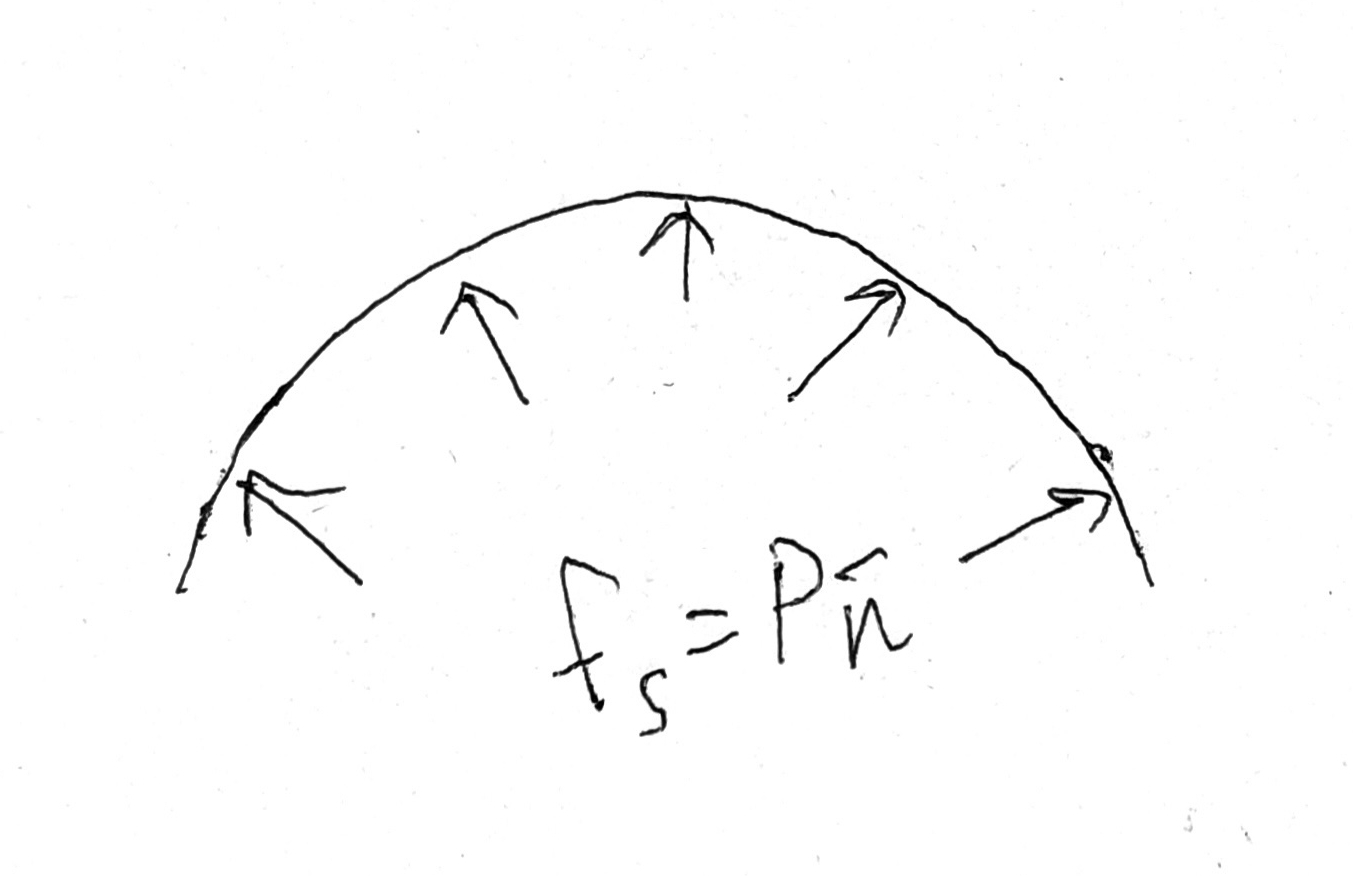
\includegraphics[width=0.5\textwidth]{fs.jpg}
    \caption{}
    \label{fig:myimage} 
\end{figure}
\begin{figure}[H] 
    \centering
    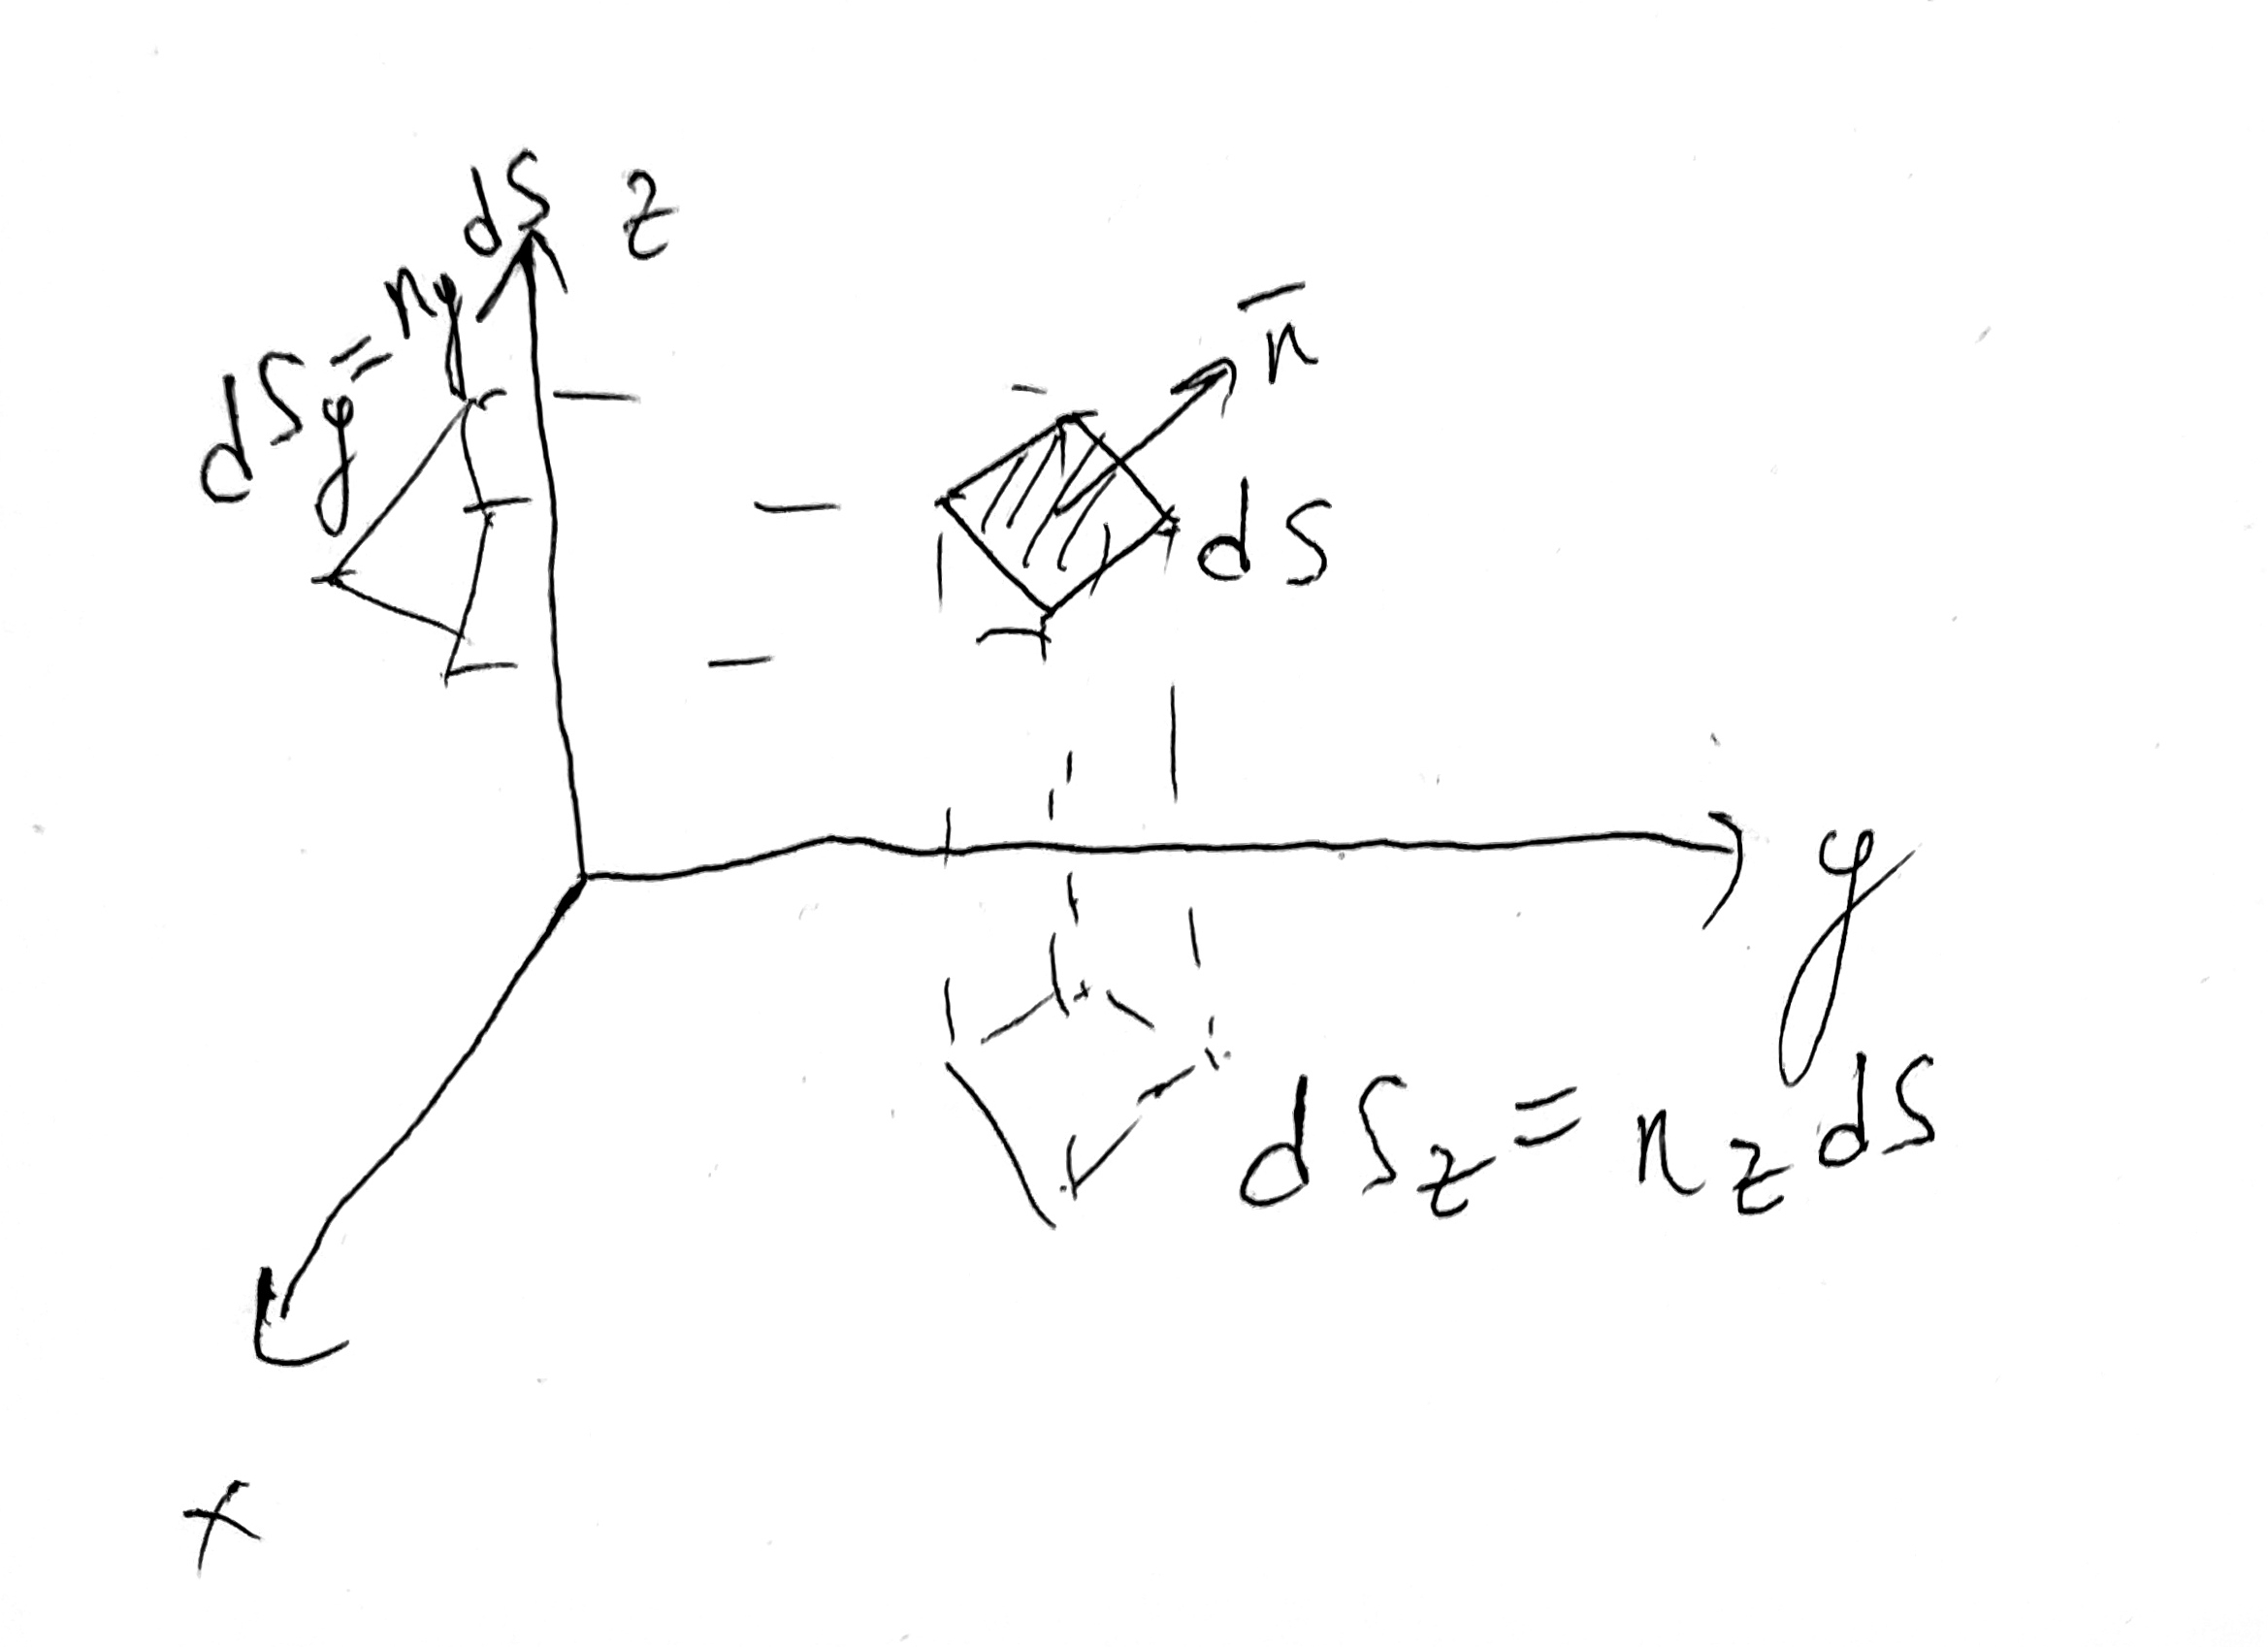
\includegraphics[width=0.5\textwidth]{videli.jpg}
    \caption{}
    \label{fig:myimage} 
\end{figure}
\[\bar R = \int_\sigma \bar f_s d s = \int_\sigma P \bar n d s = P \int_\sigma \bar n d s = P \begin{pmatrix}
    \int_\sigma n_x d s \\ \int_\sigma n_y d s \\ \int_\sigma n_z d s
\end{pmatrix} = P \begin{pmatrix}
    \int_\sigma d s_x \\ \int_\sigma d s_y \\ \int_\sigma d s_z
\end{pmatrix} = P \begin{pmatrix}
S_x \\ S_y \\ S_z
\end{pmatrix}
\]
Такие площади $S_x, S_y, S_z$ — называются площадями виделей

\keypoint
\[\bar J_{\bar u} = \sum_{k=1}^{N} m_k \rho_k^2  = \sum_{k=1}^{N} m_k(r_k^2 - (\bar r_k, \bar u)^2) = \int_S (r^2 - (\bar r, \bar u)^2) d m\]
Упр: переписать получаемые утверждения в непрерывном виде
\[\bar r_k = \begin{pmatrix}
    x_k \\ y_k \\ z_k
\end{pmatrix} \qquad \bar u = \begin{pmatrix}
    \alpha \\ \beta \\ \gamma
\end{pmatrix}\]
\[
\begin{aligned}
J_{\bar u} &= \sum_{k=1}^{N} m_k (x_k^2 + y_k^2 + z_k^2 - (\alpha x_k + \beta y_k + \gamma z_k)^2) \\
& = \sum_{k=1}^{N} m_k( x_k^2 + y_k^2 + z_k^2 - \alpha^2 x_k^2 - \beta^2 y_k^2  - \gamma^2 z_k^2 - 2 \alpha \beta x_k y_k - 2 \alpha \gamma x_k z_k - 2\beta \gamma y_k z_k)\\
& \qquad \Bigg|\alpha^2 + \beta^2 + \gamma^2 = 1\Bigg| \\
&= \sum_{k=1}^{N} (x_k^2 ( \beta^2 + \gamma^2)+ y_k^2 (\alpha^2 + \beta^2) + z_k^2 ( \beta^2 + \gamma^2)  - 2 \alpha \beta x_k y_k - 2 \alpha \gamma x_k z_k - 2\beta \gamma y_k z_k) m_k \\
&= \alpha^2 \sum_{k=1}^{N} m_k(y_k^2 + z_k^2) + \beta^2 \sum_{k=1}^{N} m_k (x_k^2 + z_k^2) + \gamma^2 \sum_{k=1}^{N} m_k(y_k^2 + x_k^2) - 2 \alpha \beta \sum_{k=1}^{N} m_k x_k y_k - 2 \beta \gamma\sum_{k=1}^{N} y_k z_k - 2 \alpha \gamma \sum_{k=1}^{N} m_k x_k z_k \\
&= \alpha^2 J_x + \beta^2 J_y + \gamma^2 J_z - 2 \alpha \beta J_{x y} - 2 \alpha \gamma J_{x z} - 2 \beta \gamma J_{y z} = \bar u^T J \bar u
\end{aligned}
\] % fixme
Тензор инерции:
\[J = \begin{pmatrix}
    J_x & - J_{x y} & - J_{x z} \\
    - J_{x y} & J_y & - J_{y z} \\
    - J_{x z} & J_{z y} & J_z
\end{pmatrix} \qquad J_{\bar u} = \bar u^T J \bar u\]
$J_{x y}$ называются центробежными моментами инерции

Тензор потому что инвариантен повороту
\end{document}